% !TeX spellcheck = en_GB
% ***************************************************** %
\section{Experiments and results discussion}\label{sc:exp}
% ***************************************************** %

%\begin{table}
%\caption[]{Hyper-parameters}
%\label{tab:hyper-params}
%\[
%\begin{array}{l}
%\beta=0.9 \\
%\end{array}
%\]
%\end{table}

%\begin{figure}
%\centering
%\includegraphics[width=0.3\textwidth]{../py/test.pdf}
%\end{figure}

% df.to_latex

To test the efficiency the algorithms, a benchmark of six datasets retrieved from \href{https://www.csie.ntu.edu.tw/~cjlin/libsvmtools/datasets/}{LIBSVM} is used, see table~\vref{tab:datasets} for details.

First the six algorithms are tested on a fixed number of epochs, \textcite{fan_msl_2023} set the value to \num{200}, so we do the same. We keep track of the loss function value for every epoch and the running time that every epoch took; our aim is to show how the value decreases on every epoch and the running time that takes, see figures on pages~\pageref{fig:diab-breast}, \pageref{fig:phish-austr} and \pageref{fig:mush-german}.\par\smallskip

Once we have the algorithms performance at different step-size values, a fine-tuning of the hyper-parameter is done in order to obtain the best solver for every dataset based on the accuracy score and loss function values. For a better comparison, the L-BFGS, Conjugate Gradient and Newton-CG, and the full-batch gradient descent algorithms are also tested.

The only hyper-parameter that varies is the step-size $\alpha$, the momentum term is set to \num{0.9}, the mini-batch size is a power of 2 and is set according to perform at least \num{100} \emph{iterations} depending on the considered dataset and the $\epsilon$ tolerance from~\eqref{eq:stopping} is set to \num{e-3}.

\begin{table}
\centering
\caption{Benchmark datasets}
\label{tab:datasets}
\begin{tabular}{lSSSc}
\toprule
Name & {Train} & {Test} & {Features} & {Distribution} \\
\midrule
w1a & 2477 & 47272 & 300 & -1:$0.97$\,\,\,1:$0.03$ \\
w3a & 4912 & 44837 & 300 & -1:$0.97$\,\,\,1:$0.03$ \\
Phishing & 8844 & 2211 & 68 & -1:$0.45$\,\,\,1:$0.55$ \\
a2a & 2265 & 30296 & 119 & -1:$0.75$\,\,\,1:$0.25$ \\
Mushrooms & 6499 & 1625 & 112 & -1:$0.48$\,\,\,1:$0.52$ \\
German & 800 & 200 & 24 & -1:$0.70$\,\,\,1:$0.30$ \\
\bottomrule
\end{tabular}
\end{table}

%\cleardoublepage
\begin{table}
\sisetup{round-mode=places}
\centering
\caption{w1a dataset}
\label{tab:w1a-table}
\begin{tabular}{lS[round-precision=3]S[drop-zero-decimal]S[round-precision=4]S[round-precision=6]S[exponent-mode=scientific]S[round-precision=6]}
\toprule
Solver & {$\alpha_0$} & {Epochs} & {Run-time} & {$\func(w)$} & {$\nabla f(w)$} & {Test score} \\
\midrule
Newton-CG & NaN & 6 & NaN & 0.464614 & 0.000046 & 0.970236 \\
CG & NaN & 7 & NaN & 0.464614 & 0.000009 & 0.970236 \\
L-BFGS-B & NaN & 7 & NaN & 0.464614 & 0.000023 & 0.970236 \\
BatchGD-Fixed & 0.750000 & 17 & 0.014591 & 0.464614 & 0.000791 & 0.970236 \\
SGD-Decreasing & 1.000000 & 85 & 1.155595 & 0.464615 & 0.000973 & 0.970236 \\
SGDM & 0.050000 & 94 & 1.274373 & 0.464615 & 0.000989 & 0.970236 \\
SGD-Fixed & 0.005000 & 41 & 0.546509 & 0.464615 & 0.000970 & 0.970236 \\
MSL-SGDM-C & 0.500000 & 600 & 12.908739 & 0.466033 & 0.042922 & 0.970236 \\
MSL-SGDM-R & 0.500000 & 600 & 12.890633 & 0.466033 & 0.042922 & 0.970236 \\
SGD-Armijo & 0.050000 & 600 & 12.424554 & 0.483484 & 0.145005 & 0.970236 \\
\bottomrule
\end{tabular}
\end{table}

\begin{table}
\sisetup{round-mode=places}
\centering
\caption{w3a dataset}
\label{tab:w3a-tab}
\begin{tabular}{lS[round-precision=3]S[drop-zero-decimal]S[round-precision=4]S[round-precision=6]S[exponent-mode=scientific]S[round-precision=6]}
\toprule
Solver & {$\alpha_0$} & {Epochs} & {Run-time} & {$\func(w)$} & {$\nabla f(w)$} & {Test score} \\
\midrule
Newton-CG & NaN & 6 & NaN & 0.462742 & 0.000011 & 0.970203 \\
CG & NaN & 7 & NaN & 0.462742 & 0.000022 & 0.970203 \\
L-BFGS-B & NaN & 7 & NaN & 0.462742 & 0.000033 & 0.970203 \\
BatchGD-Fixed & 0.750000 & 17 & 0.018317 & 0.462743 & 0.000791 & 0.970203 \\
SGD-Fixed & 0.005000 & 42 & 0.574441 & 0.462743 & 0.000850 & 0.970203 \\
SGD-Decreasing & 1.000000 & 72 & 1.006146 & 0.462743 & 0.000989 & 0.970203 \\
SGDM & 0.040000 & 99 & 1.361420 & 0.462743 & 0.000970 & 0.970203 \\
MSL-SGDM-C & 0.500000 & 600 & 12.062421 & 0.463348 & 0.028706 & 0.970203 \\
MSL-SGDM-R & 0.750000 & 600 & 12.468809 & 0.465611 & 0.066743 & 0.970203 \\
SGD-Armijo & 0.100000 & 600 & 12.561584 & 0.472486 & 0.111806 & 0.970203 \\
\bottomrule
\end{tabular}
\end{table}

\begin{table}
\sisetup{round-mode=places}
\caption{Phishing dataset}
\label{tab:phish-tab}
\centering
\begin{tabular}{lS[round-precision=3]S[drop-zero-decimal]S[round-precision=4]S[round-precision=6]S[exponent-mode=scientific]S[round-precision=6]}
\toprule
Solver & {$\alpha_0$} & {Epochs} & {Run-time} & {$\func(w)$} & {$\nabla f(w)$} & {Test score} \\
\midrule
Newton-CG & NaN & 5 & NaN & 0.685065 & 0.000000 & 0.567616 \\
L-BFGS-B & NaN & 5 & NaN & 0.685065 & 0.000008 & 0.567616 \\
CG & NaN & 6 & NaN & 0.685065 & 0.000023 & 0.567616 \\
SGD-Decreasing & 1.000000 & 31 & 0.421835 & 0.685065 & 0.000660 & 0.567616 \\
SGD-Fixed & 0.010000 & 21 & 0.273023 & 0.685065 & 0.000847 & 0.567616 \\
BatchGD-Fixed & 0.500000 & 25 & 0.063251 & 0.685065 & 0.000829 & 0.567616 \\
SGDM & 0.050000 & 79 & 1.064213 & 0.685065 & 0.000880 & 0.567616 \\
MSL-SGDM-C & 0.500000 & 600 & 13.559572 & 0.685705 & 0.032668 & 0.568973 \\
MSL-SGDM-R & 0.500000 & 600 & 12.843879 & 0.686124 & 0.043719 & 0.567616 \\
SGD-Armijo & 0.010000 & 600 & 11.481668 & 0.703591 & 0.182149 & 0.567616 \\
\bottomrule
\end{tabular}
\end{table}

\begin{table}
\sisetup{round-mode=places}
\caption{a2a dataset}
\label{tab:a2a-tab}
\centering
\begin{tabular}{lS[round-precision=3]S[drop-zero-decimal]S[round-precision=4]S[round-precision=6]S[exponent-mode=scientific]S[round-precision=6]}
\toprule
Solver & {$\alpha_0$} & {Epochs} & {Run-time} & {$\func(w)$} & {$\nabla f(w)$} & {Test score} \\
\midrule
Newton-CG & NaN & 5 & NaN & 0.564027 & 0.000004 & 0.760265 \\
CG & NaN & 12 & NaN & 0.564027 & 0.000015 & 0.760265 \\
L-BFGS-B & NaN & 8 & NaN & 0.564027 & 0.000012 & 0.760265 \\
BatchGD-Fixed & 0.500000 & 26 & 0.020425 & 0.564028 & 0.000756 & 0.760265 \\
SGDM & 0.020000 & 210 & 2.468821 & 0.564028 & 0.000917 & 0.760265 \\
SGD-Fixed & 0.001000 & 208 & 2.479476 & 0.564028 & 0.000986 & 0.760265 \\
SGD-Decreasing & 0.050000 & 34 & 0.406210 & 0.564028 & 0.000994 & 0.760265 \\
MSL-SGDM-R & 0.100000 & 600 & 11.812484 & 0.566102 & 0.075915 & 0.761157 \\
MSL-SGDM-C & 0.100000 & 600 & 12.078144 & 0.566957 & 0.085563 & 0.768022 \\
SGD-Armijo & 0.010000 & 600 & 12.179206 & 0.572869 & 0.123547 & 0.764820 \\
\bottomrule
\end{tabular}
\end{table}

\begin{table}
\sisetup{round-mode=places}
\caption{Mushrooms dataset}
\label{tab:mush-tab}
\centering
\begin{tabular}{lS[round-precision=3]S[drop-zero-decimal]S[round-precision=4]S[round-precision=6]S[exponent-mode=scientific]S[round-precision=6]}
\toprule
Solver & {$\alpha_0$} & {Epochs} & {Run-time} & {$\func(w)$} & {$\nabla f(w)$} & {Test score} \\
\midrule
Newton-CG & NaN & 7 & NaN & 0.517726 & 0.000003 & 0.892923 \\
CG & NaN & 11 & NaN & 0.517726 & 0.000024 & 0.892923 \\
L-BFGS-B & NaN & 10 & NaN & 0.517726 & 0.000017 & 0.892923 \\
SGD-Decreasing & 0.100000 & 13 & 0.124991 & 0.517727 & 0.000622 & 0.892923 \\
SGDM & 0.030000 & 192 & 1.855943 & 0.517727 & 0.000903 & 0.892923 \\
SGD-Fixed & 0.001000 & 289 & 2.814241 & 0.517727 & 0.000988 & 0.892923 \\
BatchGD-Fixed & 0.050000 & 285 & 0.448186 & 0.517727 & 0.000997 & 0.892923 \\
MSL-SGDM-R & 0.025000 & 600 & 9.859336 & 0.518412 & 0.043708 & 0.892923 \\
MSL-SGDM-C & 0.025000 & 600 & 10.088218 & 0.519080 & 0.073248 & 0.887385 \\
SGD-Armijo & 0.010000 & 600 & 10.140186 & 0.521178 & 0.066312 & 0.889231 \\
\bottomrule
\end{tabular}
\end{table}

\begin{table}
\sisetup{round-mode=places}
\caption{German dataset}
\label{tab:german-tab}
\centering
\begin{tabular}{lS[round-precision=3]S[drop-zero-decimal]S[round-precision=4]S[round-precision=6]S[exponent-mode=scientific]S[round-precision=6]}
\toprule
Solver & {$\alpha_0$} & {Epochs} & {Run-time} & {$\func(w)$} & {$\nabla f(w)$} & {Test score} \\
\midrule
Newton-CG & NaN & 5 & NaN & 0.597303 & 0.000010 & 0.710000 \\
CG & NaN & 12 & NaN & 0.597303 & 0.000004 & 0.710000 \\
L-BFGS-B & NaN & 7 & NaN & 0.597303 & 0.000014 & 0.710000 \\
SGD-Decreasing & 0.250000 & 42 & 0.361343 & 0.597303 & 0.000700 & 0.710000 \\
BatchGD-Fixed & 0.500000 & 20 & 0.010634 & 0.597303 & 0.000882 & 0.710000 \\
SGDM & 0.010000 & 482 & 4.061424 & 0.597303 & 0.000974 & 0.710000 \\
SGD-Fixed & 0.001000 & 231 & 1.970545 & 0.597303 & 0.000985 & 0.710000 \\
MSL-SGDM-R & 0.500000 & 600 & 8.571129 & 0.601524 & 0.090918 & 0.705000 \\
MSL-SGDM-C & 0.500000 & 600 & 8.865525 & 0.619598 & 0.269061 & 0.700000 \\
SGD-Armijo & 0.050000 & 600 & 9.004771 & 0.892683 & 0.978264 & 0.705000 \\
\bottomrule
\end{tabular}
\end{table}

\begin{figure}
\centering
% w1a
\subfloat[][\emph{w1a dataset}\label{subfig:w1a-diagnostic}]%
{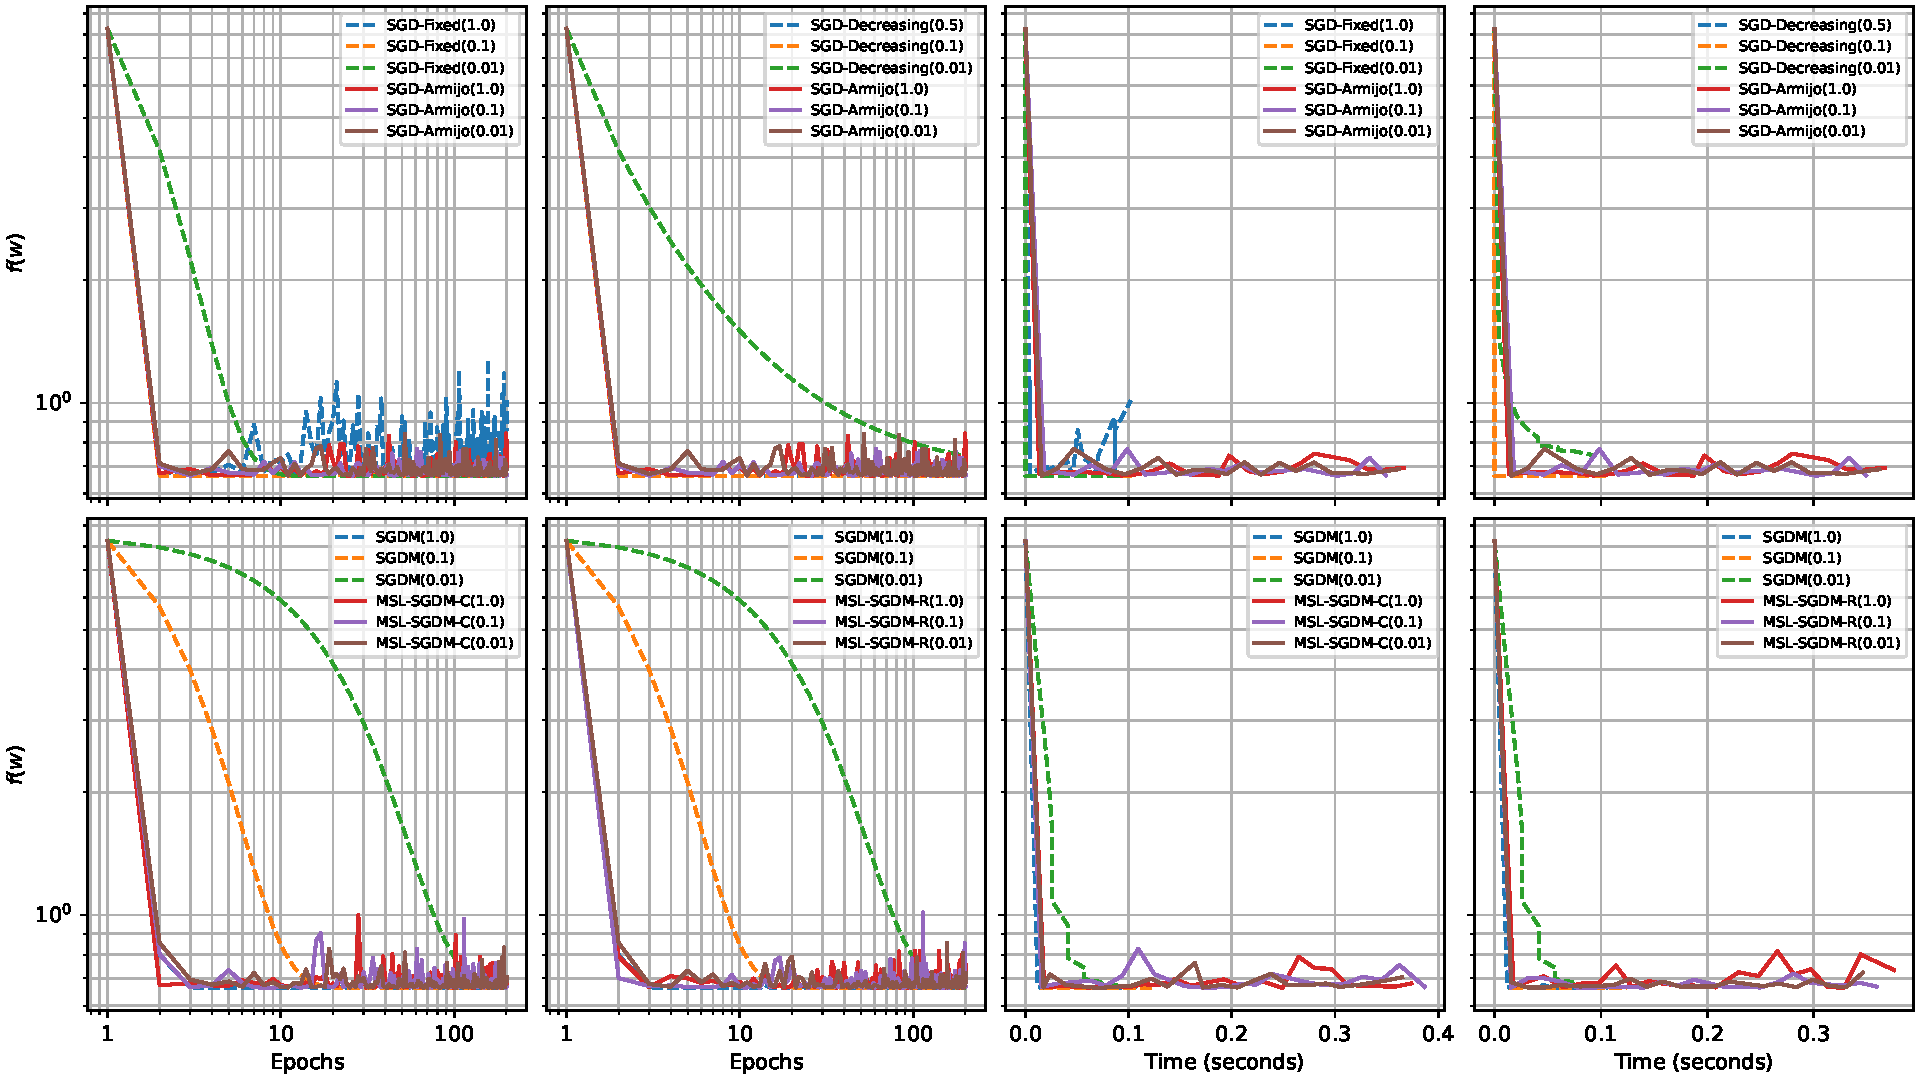
\includegraphics[width=\textwidth]{diab-diagnostic}} \\
% w3a
\subfloat[][\emph{w3a dataset}\label{subfig:w3a-diagnostic}]%
{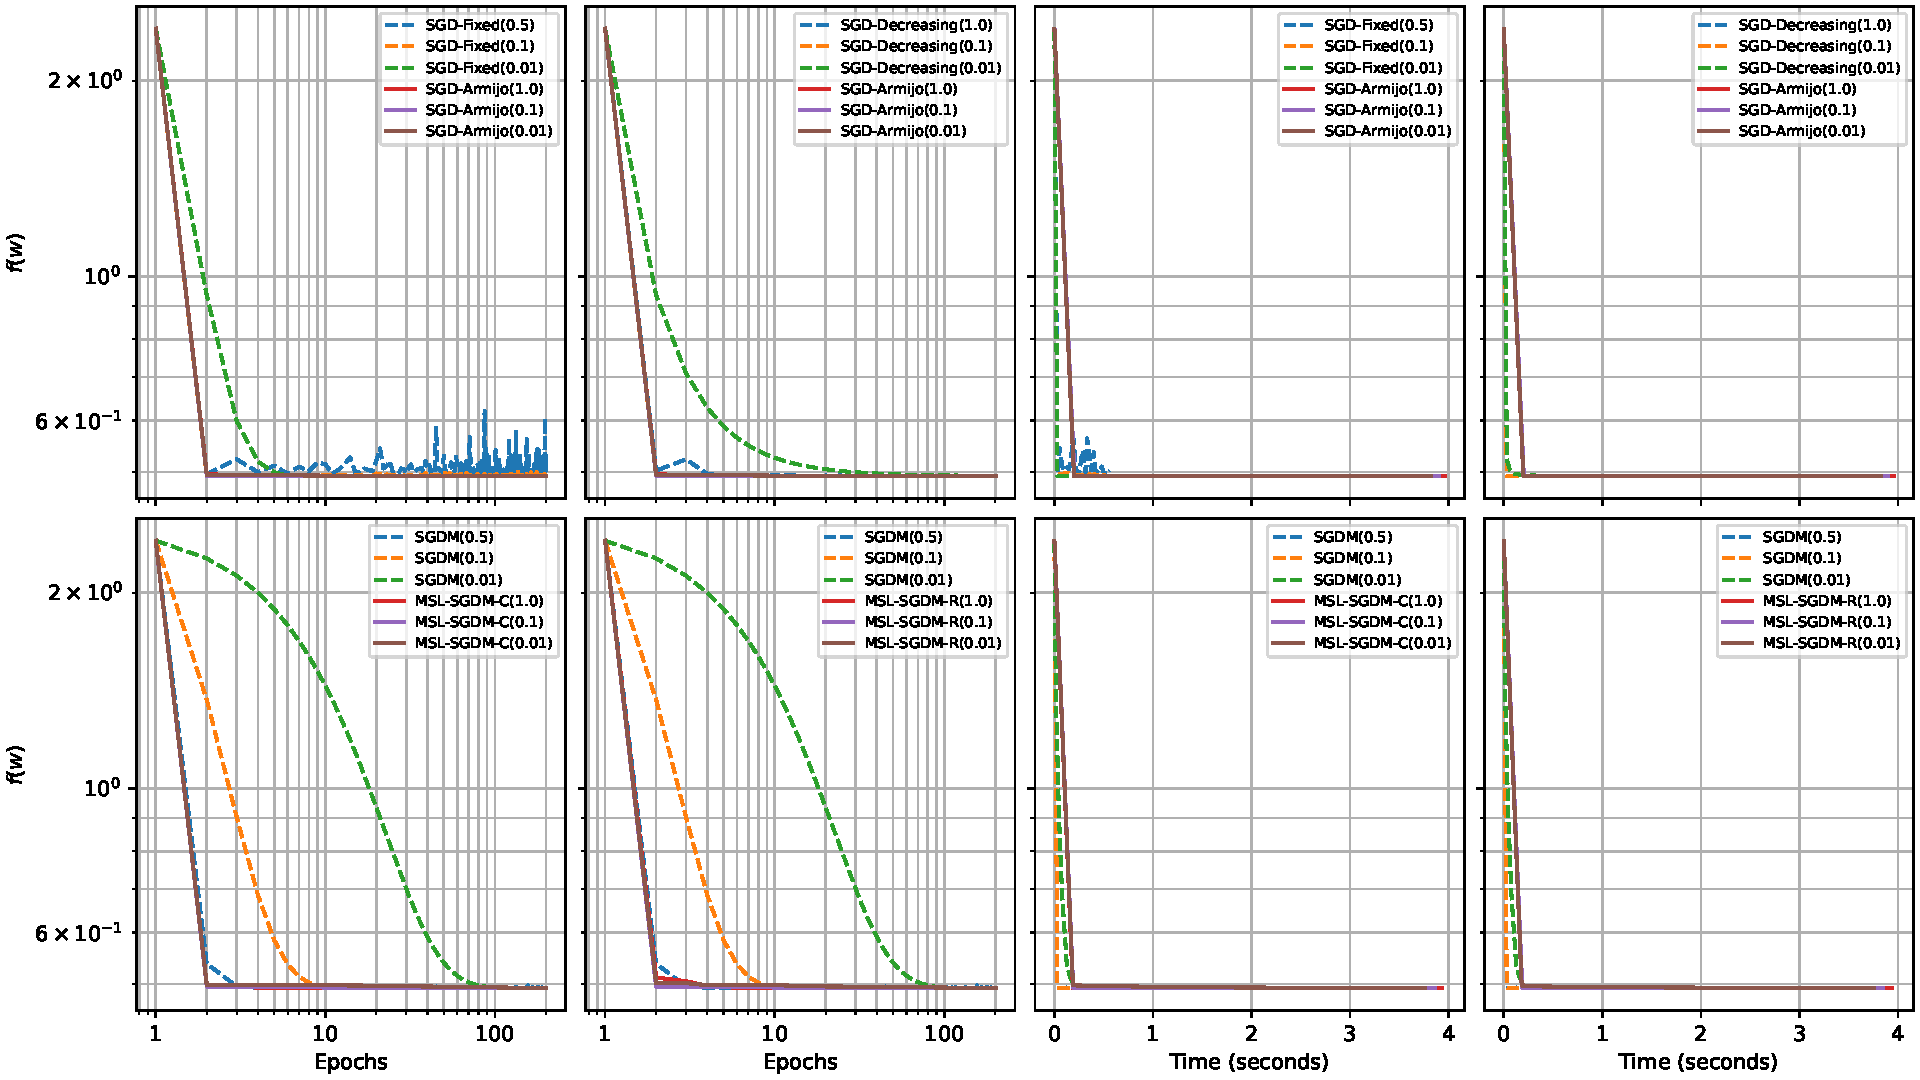
\includegraphics[width=\textwidth]{breast-diagnostic}} \\
\caption[]{w1a and w3ar}
\label{fig:diab-breast}
\end{figure}

\begin{figure}
\centering
% Phishing
\subfloat[][\emph{Phishing dataset}\label{subfig:phish-diagnostic}]%
{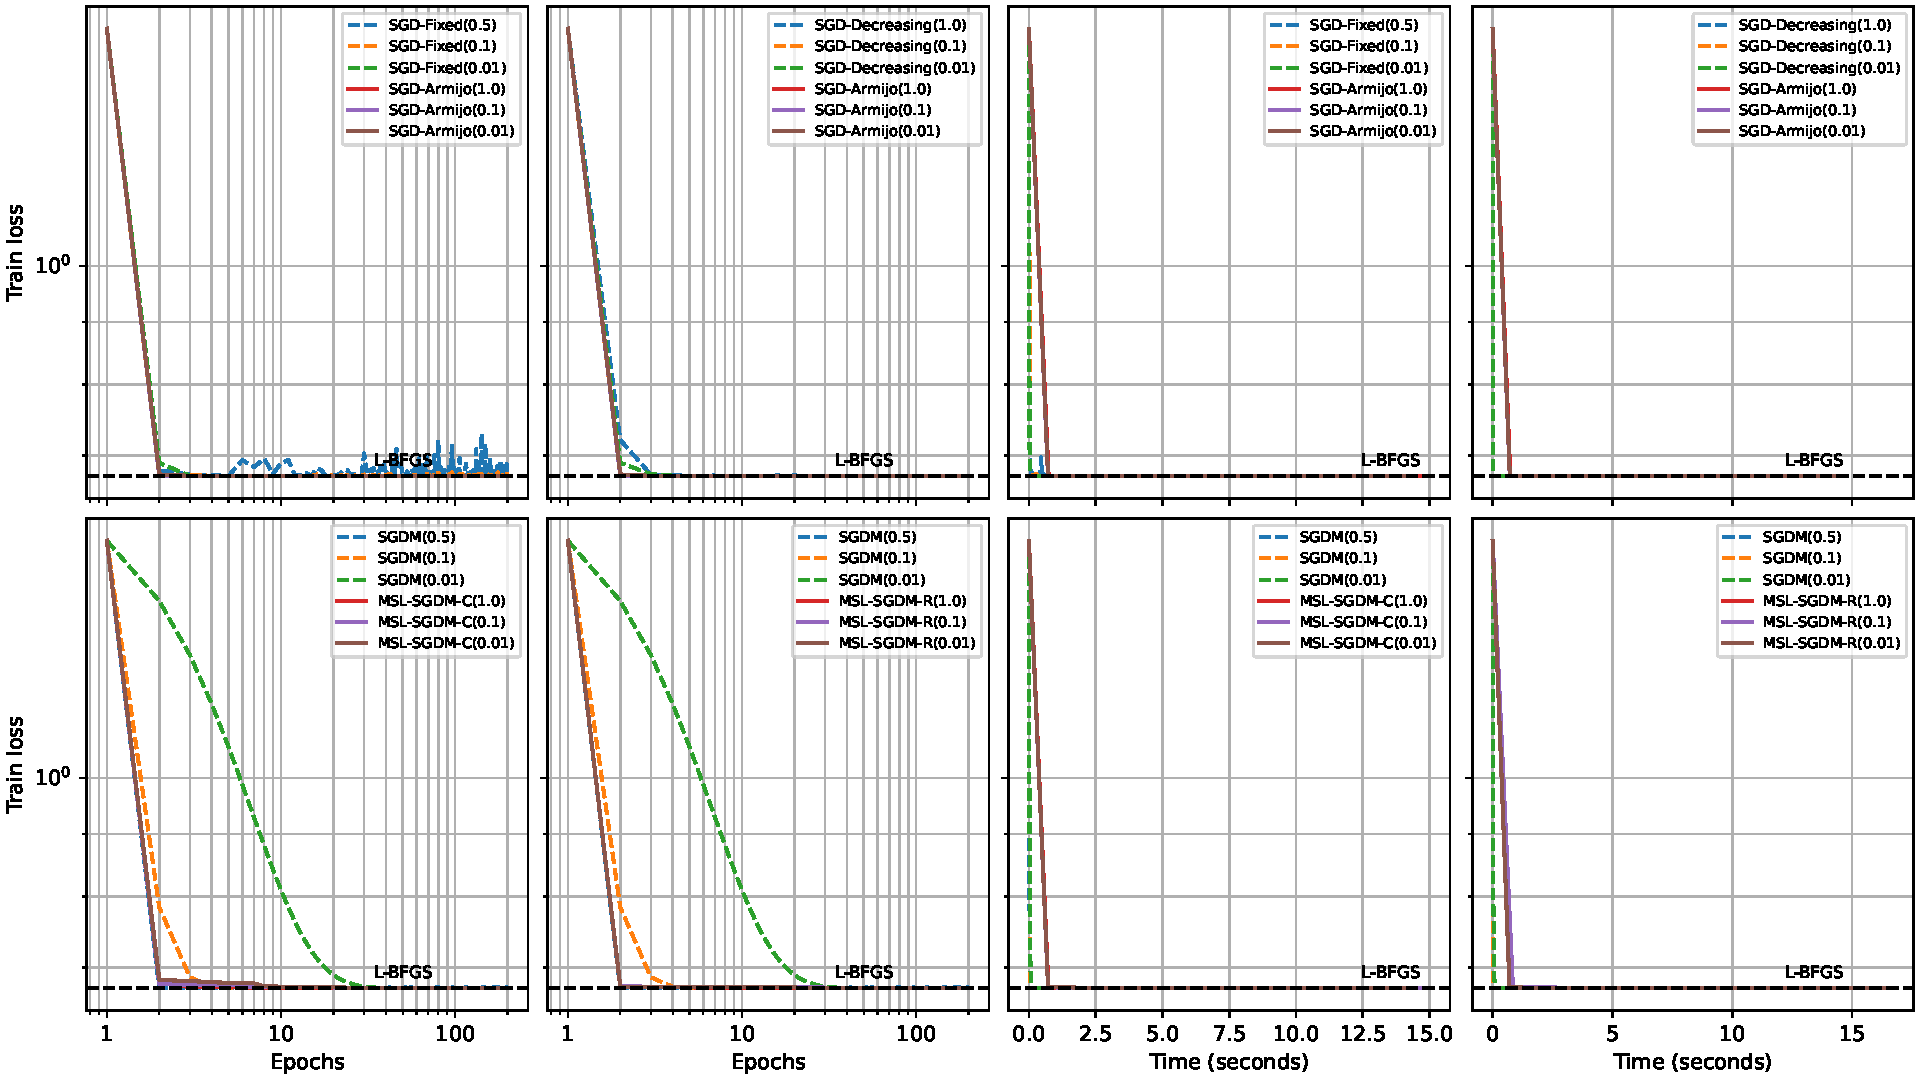
\includegraphics[width=\textwidth]{svm-diagnostic}} \\
% a2a
\subfloat[][\emph{a2a dataset}\label{subfig:a2a-diagnostic}]%
{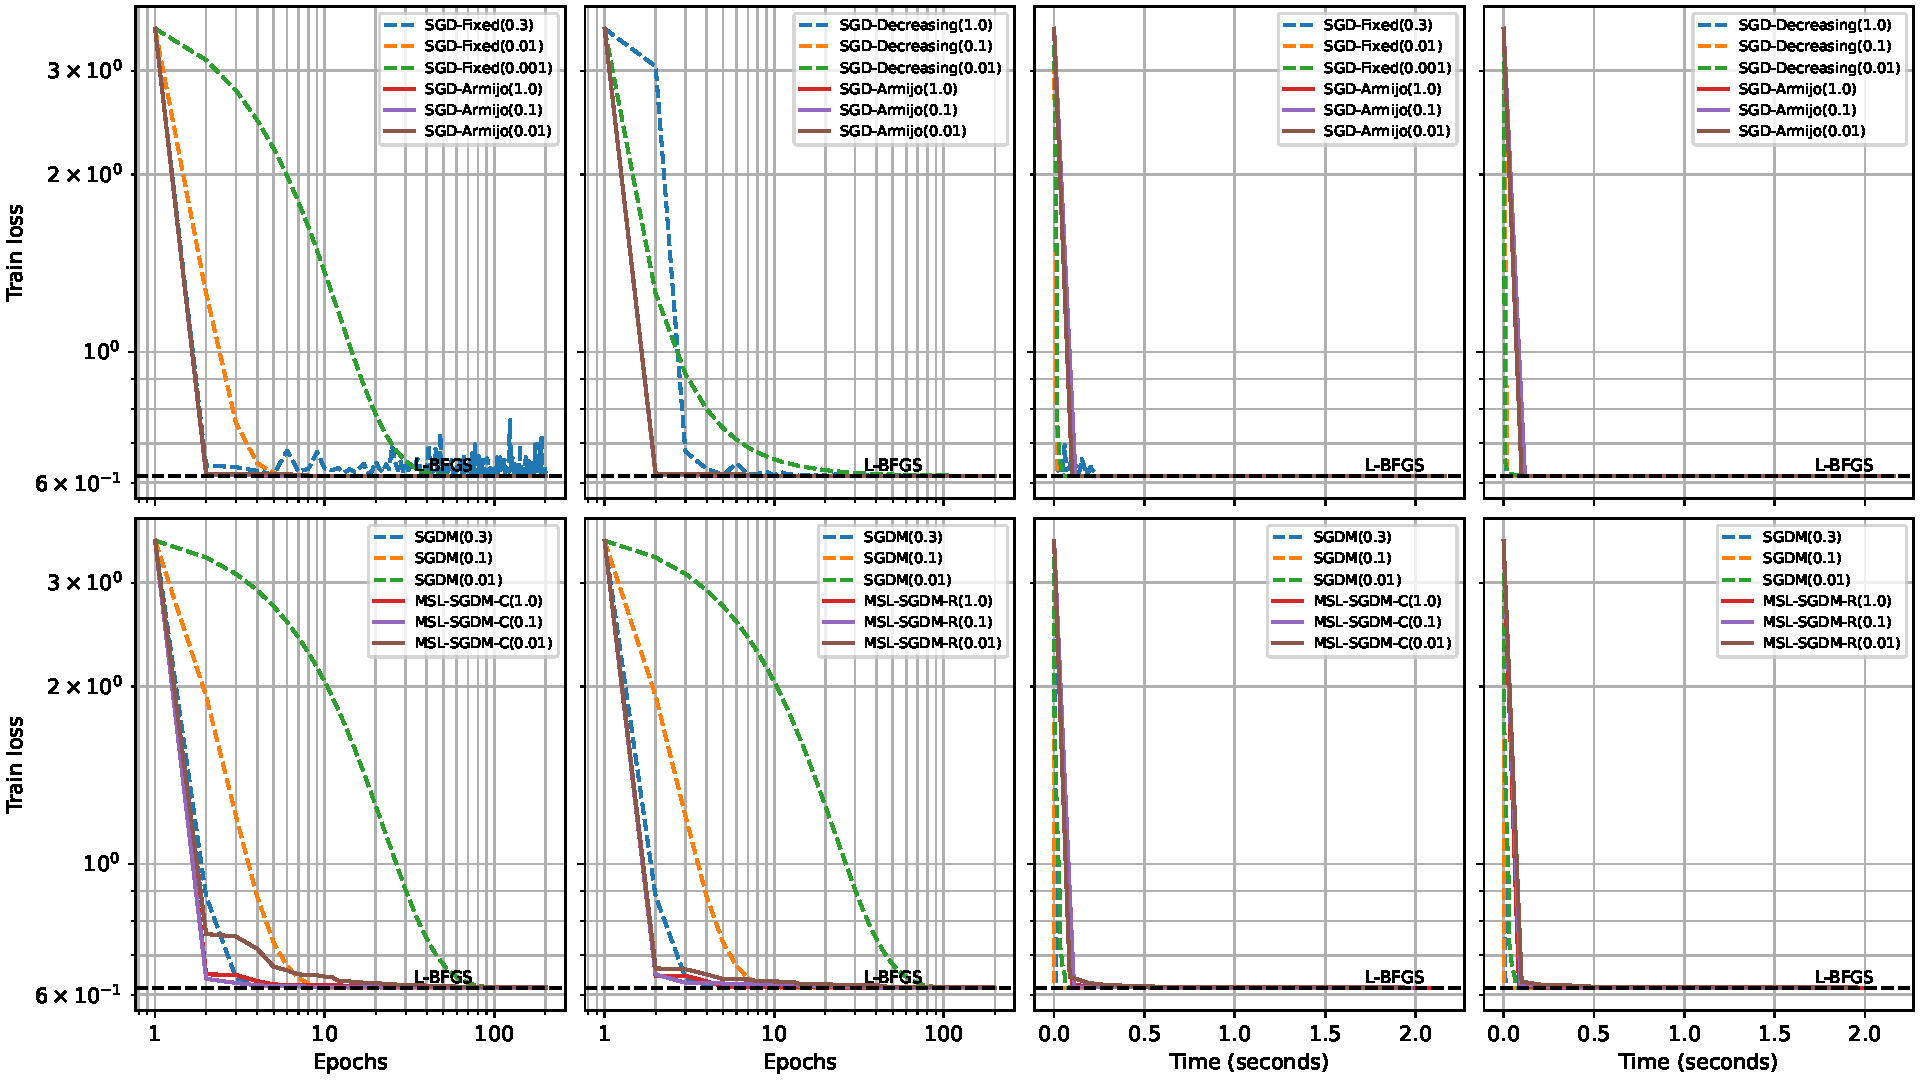
\includegraphics[width=\textwidth]{austr-diagnostic}}
\caption[]{Phishing and a2a datasets}
\label{fig:phish-austr}
\end{figure}

\begin{figure}
\centering
% mushrooms
\subfloat[][\emph{Mushrooms dataset}\label{subfig:mush-diagnostic}]%
{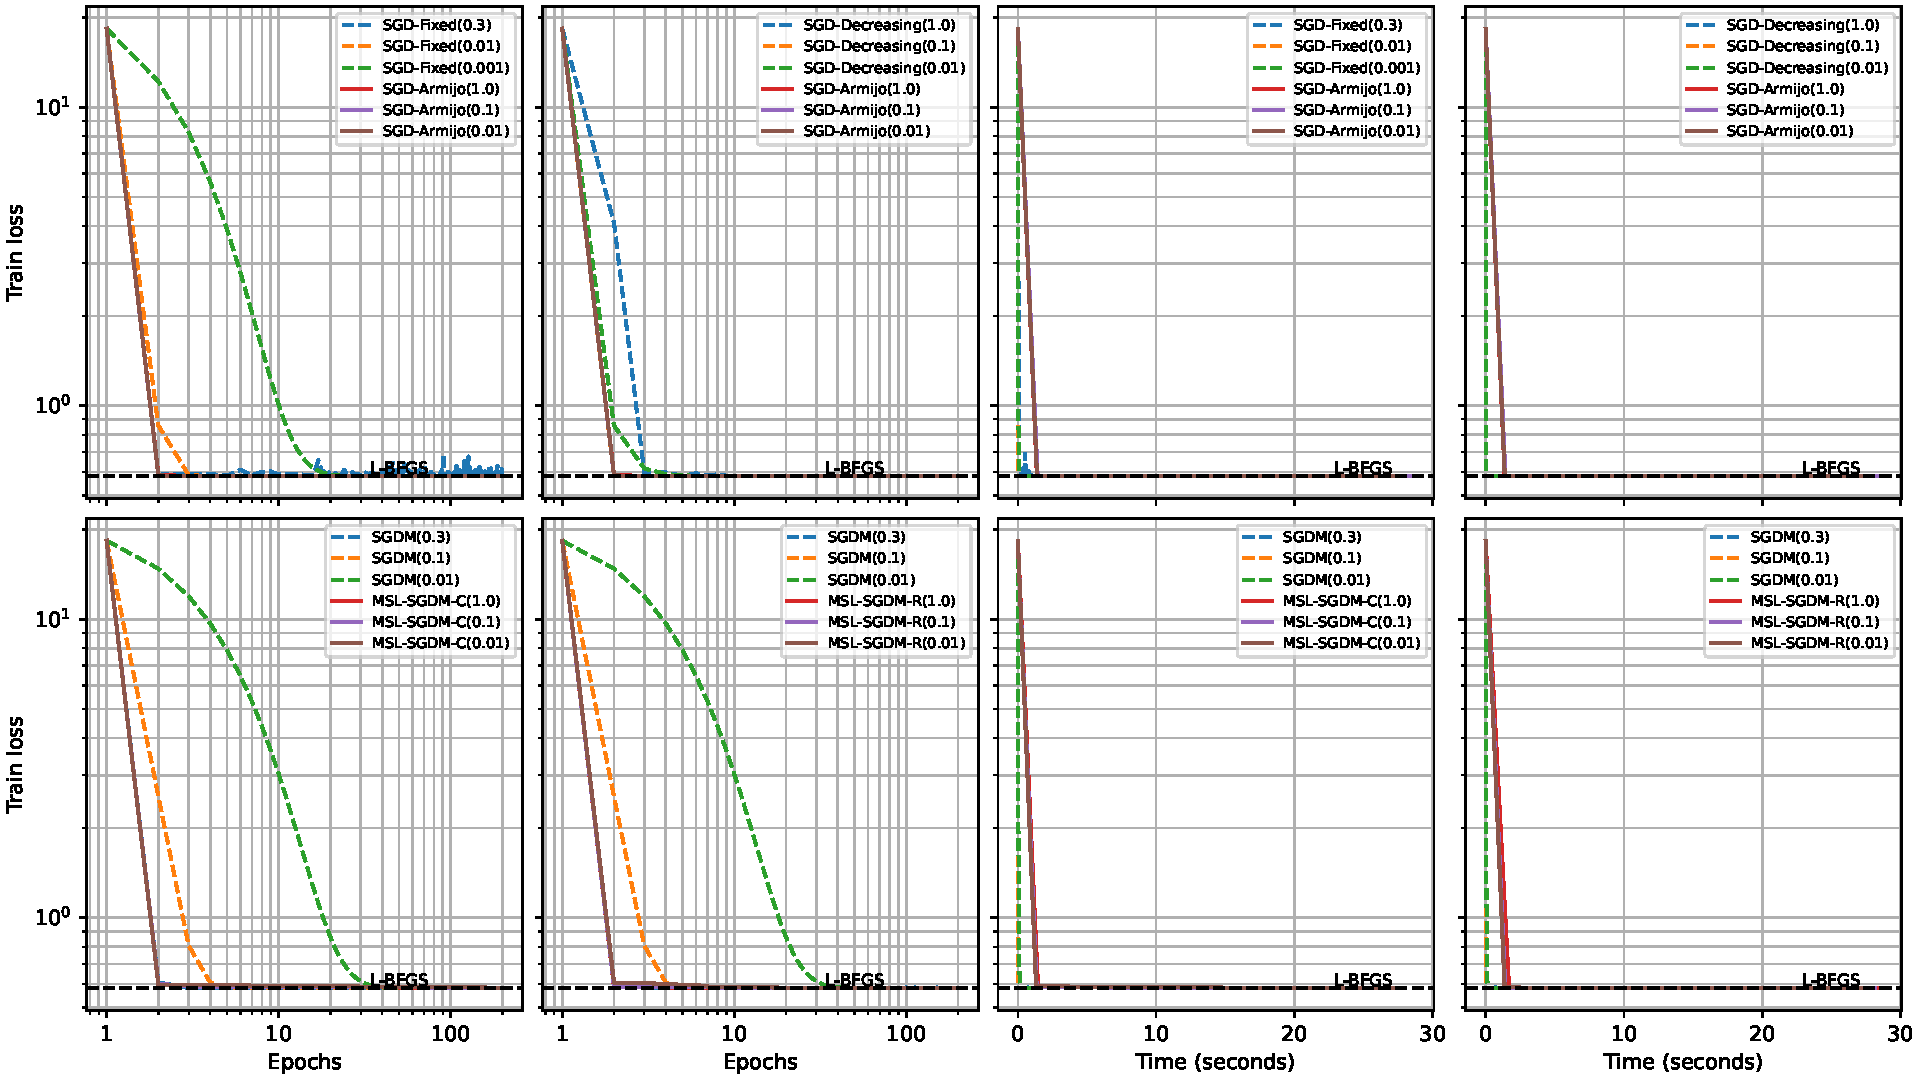
\includegraphics[width=\textwidth]{mush-diagnostic}} \\
% german
\subfloat[][\emph{German dataset}\label{subfig:german-diagnostic}]%
{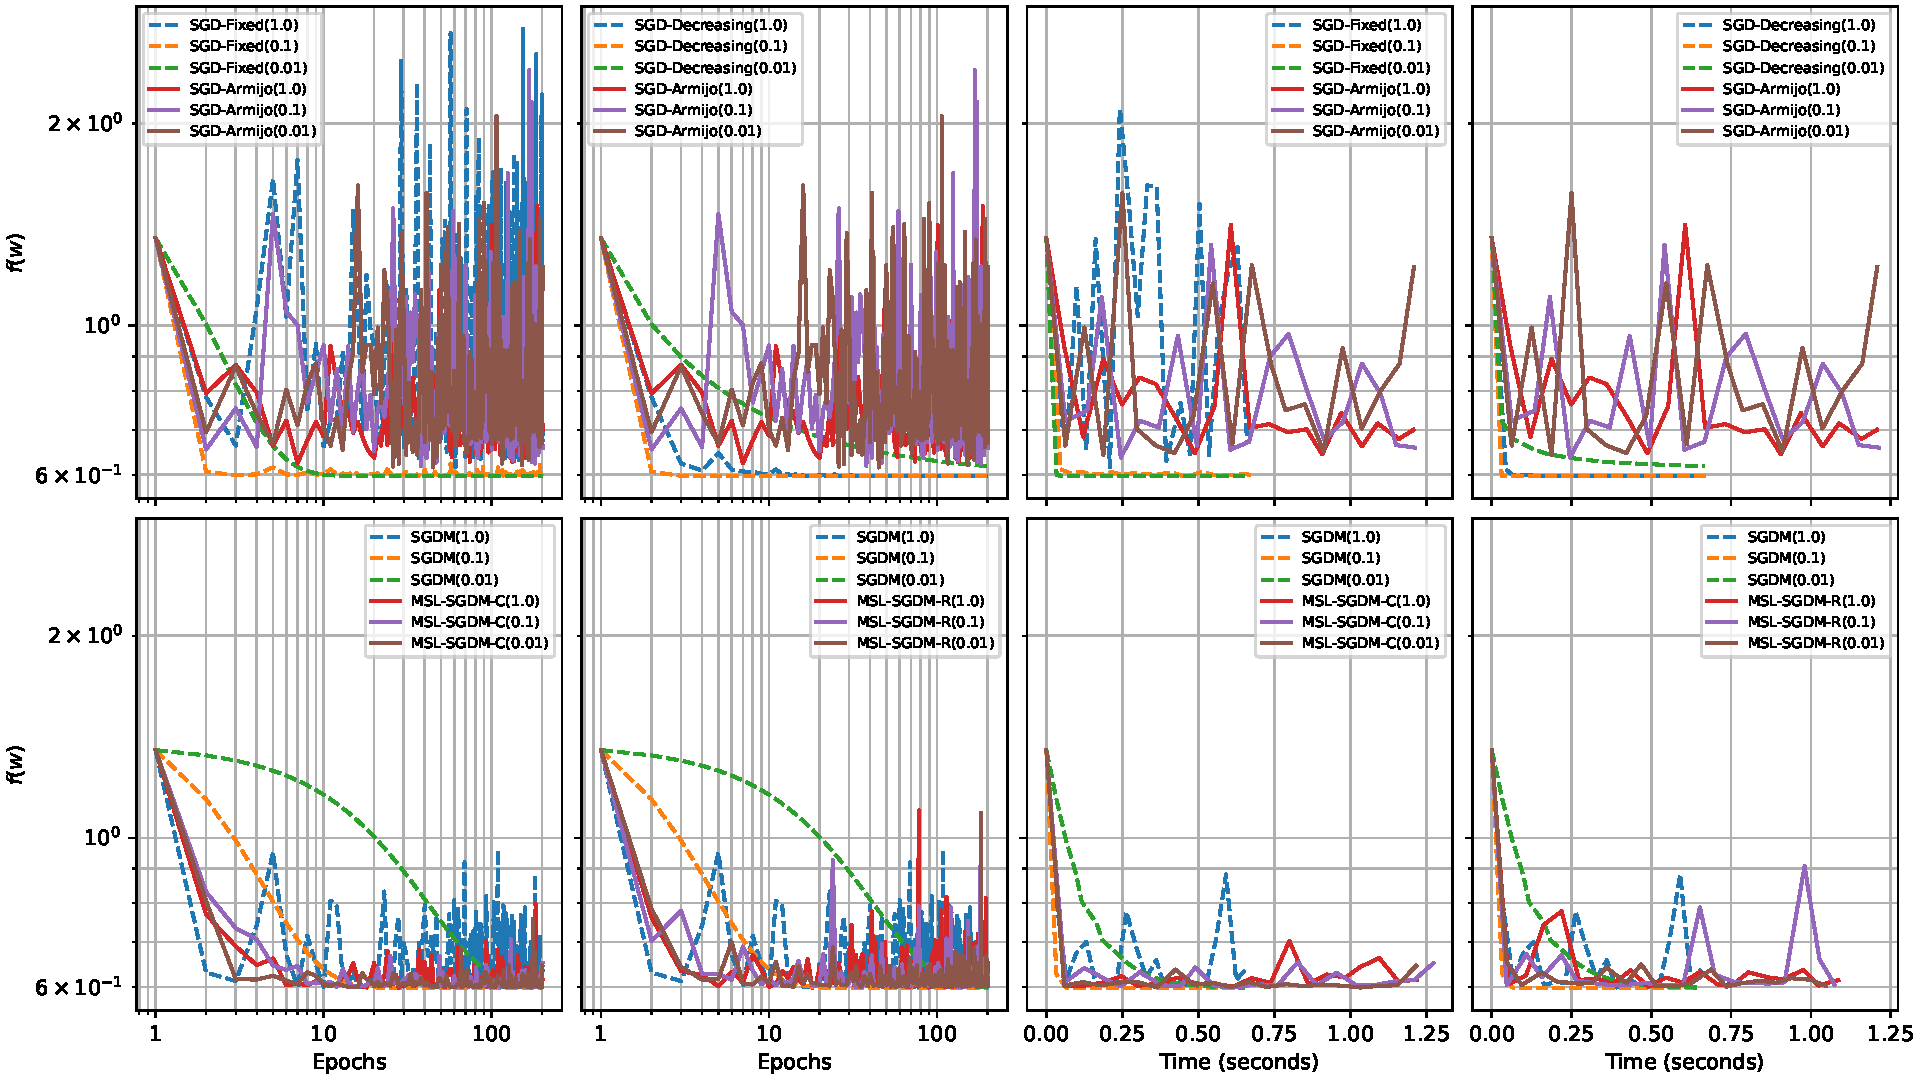
\includegraphics[width=\textwidth]{german-diagnostic}}
\caption[]{Mushrooms and German datasets}
\label{fig:mush-german}
\end{figure}

%\cleardoublepage
% ***************************************************** %
%\section{Mathematical background}
% ***************************************************** %

%\begin{defs}[Convex function]\label{def:conv_fun}
%	Let $S\subseteq\R^n$ be a convex set, a function $f\colon S\to\R$ is said to be convex if the hessian matrix is semi-positive-defined. If the hessian matrix is positive-defined, then the function is strictly convex.
%\end{defs}
%
%\begin{thm}[Weirstrass theorem]\label{thm:weirs}
%	Let $f\colon\R^n\to\R$ be a continuous function and $S\subseteq\R^n$ a compact set. Then function $f$ admits global minimum in $S$.
%\end{thm}
%
%\begin{cor}[Sufficient condition]\label{cor:weirs1}
%	If function $f\colon\R^n\to\R$ is a continuous and coercive function, then $f$ admits global minimum in $\R^n$.
%\end{cor}
%
%\begin{prop}[Coercivity of a quadratic function]
%	A quadratic function $\func(x)=\frac{1}{2}x^TQx-c^Tx$ is said to be coercive if and only if the symmetric matrix $Q\in\R^{n\times n}$ is positive-defined.
%\end{prop}
%
%\begin{prop}[Unique global minimum]\label{prop:min_unique}
%	Let $S\subseteq\R^n$ be a convex set, let $f\colon S\to\R$ be a strictly convex function. Then the global minimum, if exists, is unique.
%\end{prop}
%
%\begin{prop}[First order optimality condition]
%	$\bar{x}$ is a local minimum for $f\colon\R^n\to\R$ of class $f\in C^1(\R^n)$ if and only if $\nabla\func(\bar{x})=0$.
%\end{prop}
%
%\begin{prop}[Second order optimality condition]\label{prop:opt_second}
%	$\bar{x}\in\R^n$ is a local minimum for $f\colon\R^n\to\R$ of class $f\in C^2(\R^n)$ if and only if
%	\[\nabla\func(\bar{x})=0\quad\wedge\quad \nabla^2\func(\bar{x})\,\,\,\text{positive semi-definite}\]
%\end{prop}

% add definition of coercive function and proposition about compact sets?
% add gradient descent?
